\documentclass[conference]{IEEEtran}
\usepackage{cite,amsmath,amssymb,amsfonts,amsthm}
\usepackage{algorithmic,graphicx,textcomp,xcolor,booktabs,siunitx}
\usepackage{subcaption,url,hyperref,tikz}
\usetikzlibrary{arrows.meta,positioning,shapes.geometric,fit,backgrounds}
\hypersetup{colorlinks=true,linkcolor=black,citecolor=black,urlcolor=black}
\newtheorem{theorem}{Theorem}
\newtheorem{lemma}[theorem]{Lemma}
\newtheorem{definition}{Definition}
\def\BibTeX{{\rm B\kern-.05em{\sc i\kern-.025em b}\kern-.08em T\kern-.1667em\lower.7ex\hbox{E}\kern-.125emX}}

\begin{document}

\title{Deterministic and Learned Resilience in CRDT-Based\\
       Wireless Mesh Networks Under Physical Degradation:\\
       Design, Evaluation, and Phase-Transition Analysis}

\author{
  \IEEEauthorblockN{Aaditya Binod Yadav}
  \IEEEauthorblockA{Department of Computer Science\
  Kathmandu, Nepal\
  aadityabinodyadav@gmail.com}
}
\maketitle

%% ─── ABSTRACT ─────────────────────────────────────────────────────────────
\begin{abstract}
Infrastructure-less wireless mesh networks must sustain reliable message
delivery under physical channel degradation, dynamic topology, and arbitrary
network partitions---conditions that defeat both classical consensus protocols
and conventional unicast routing.  This paper presents a hybrid framework
combining \emph{deterministic} CRDT-based gossip with \emph{learned} relay
selection, and studies their joint behavior across a wireless channel phase
transition.

Our data layer formalizes an Observed-Remove Set (OR-Set) with Hybrid Logical
Clock causality and proves Strong Eventual Consistency (SEC) without
coordination.  Above this, we implement four forwarding strategies of increasing
intelligence: epidemic flooding, a hand-crafted heuristic utility function, a
regime-adaptive two-state controller, and a 12-feature logistic regression
classifier (AUC\,=\,0.69) trained on gossip traces.

Systematic evaluation across path-loss exponents $n = 2.0$--$4.5$ reveals a
sharp \emph{protocol--physics boundary}: all four strategies achieve $>$99\%
packet delivery ratio (PDR) for $n \leq 3.0$, then diverge rapidly at
$n \approx 3.5$.  The adaptive controller partially recovers the heuristic's
shortfall (83.2\%); the learned classifier degrades further (74.2\% PDR vs.\
84.9\% flooding), exhibiting topology-sensitivity under conditions outside its
training regime---a new finding quantifying a \emph{non-deterministic failure
mode} absent in deterministic strategies.

Partition analysis confirms flooding, heuristic, and adaptive satisfy the SEC
guarantee across 15--120~s outages; the learned strategy reaches 94.6\% PDR
at 120~s due to TTL expiry during relay suppression on degraded boundary links,
connecting ML relay behavior to finite-buffer CRDT invariants.  Latency grows
at $\approx$2~ms/hop; the classifier extends the observable hop distribution
to hop~7.  An ESP32 footprint projection of 6.9~KB (2.1\% SRAM) confirms
embedded viability.  Source code is available at
\url{https://github.com/aadityayadav/crdt-mesh} (upon acceptance).
\end{abstract}

\begin{IEEEkeywords}
CRDT, eventual consistency, mesh networking, gossip protocol, relay selection,
machine learning, phase transition, delay-tolerant networking,
discrete-event simulation, wireless resilience
\end{IEEEkeywords}

%% ─── I. INTRODUCTION ──────────────────────────────────────────────────────
\section{Introduction}

Modern telecommunications depend on centralized infrastructure: cell towers,
fiber backhaul, and power grids.  Natural disasters expose the fragility of this
dependency.  The 2021 Ahr Valley floods destroyed 80\% of regional cellular
coverage~\cite{itu_disaster_2022}; the 2023 Turkey-Syria earthquake left millions
without connectivity for more than 72~hours.  During such events, local
communication must operate \emph{without} any pre-existing infrastructure.

Traditional consensus protocols---Paxos~\cite{lamport_paxos_1998} and
Raft~\cite{ongaro_raft_2014}---are unsuitable here: they require stable
connectivity, elect a single-point-of-failure leader, and stall under partitions.
Conventional wireless routing (AODV~\cite{perkins_aodv_2003},
OLSR~\cite{clausen_olsr_2003}) targets point-to-point delivery, not replicated
state dissemination across dynamic topologies.

Conflict-Free Replicated Data Types~(CRDTs)~\cite{shapiro_crdt_2011} offer a
principled alternative: mathematically guaranteed convergence without coordination,
achieved through a monotone merge operator.  We adapt OR-Sets~\cite{bieniusa_or_2012}
to the constrained wireless setting and combine them with epidemic gossip and
configurable forwarding policies to address three concrete challenges:
(i)~eventual delivery under lossy wireless links,
(ii)~correct reconciliation after network partitions, and
(iii)~efficient relay selection to reduce redundant transmissions.

\subsection{Contributions}
\begin{enumerate}
  \item \textbf{Formal CRDT framework.}  OR-Set with Hybrid Logical Clock~(HLC)
        causality; SEC proved without coordination (Theorem~\ref{thm:sec}).
  \item \textbf{Four-strategy relay hierarchy.}  Epidemic flooding, hand-crafted
        heuristic, regime-adaptive controller, and a 12-feature logistic regression
        classifier, implemented in a reproducible discrete-event simulator scaling
        to 100~nodes.
  \item \textbf{Phase-transition characterization.}  First empirical mapping of
        all four strategies across path-loss exponents $n = 2.0$--$4.5$, identifying
        $n \approx 3.5$ as the protocol--physics boundary and quantifying
        per-strategy divergence across three operating regimes.
  \item \textbf{Learned strategy failure mode.}  Quantification of topology-sensitivity
        in the ML classifier: 4--9~pp PDR degradation at $n = 3.5$ and 5.4~pp PDR
        degradation under 120~s partitions, neither attributable to the deterministic
        strategies.  This constitutes a new class of failure in CRDT mesh systems.
  \item \textbf{Regime-adaptive controller.}  A two-state controller using only local
        neighbor-table signals that improves PDR by up to 4.5~pp in sparse RWP scenarios
        and establishes a local-signal observability boundary.
  \item \textbf{AODV baseline.}  Unicast comparison confirming CRDT gossip's partition
        resilience advantage (82.3\% vs.\ $>$98.8\% PDR under partition).
  \item \textbf{ESP32 footprint projection.}  6.9~KB struct layout (2.1\% of 328~KB SRAM),
        confirming protocol viability on Class-2 constrained devices.
\end{enumerate}

\subsection{Paper Organization}
Section~\ref{sec:related} surveys related work.  Sections~\ref{sec:model}--\ref{sec:crdt}
define the system and data models.  Section~\ref{sec:protocol} presents the
synchronization protocol.  Section~\ref{sec:ai} describes relay-selection strategies.
Section~\ref{sec:impl} details the implementation.  Section~\ref{sec:eval} presents
results.  Sections~\ref{sec:discuss}--\ref{sec:conclusion} discuss and conclude.

%% ─── II. RELATED WORK ─────────────────────────────────────────────────────
\section{Related Work}
\label{sec:related}

\subsection{Disaster and Emergency Communication}
Prior systems include SMESH~\cite{foo_smesh_2010} (LoRa mesh),
Serval~\cite{gardner_serval_2013} (smartphone mesh), and
Briar~\cite{briar_2019} (Tor-anonymized peer-to-peer).  These focus on
user-facing messaging but lack formal consistency guarantees and partition
recovery semantics.  Meissner et al.~\cite{meissner_dtn_rescue_2012} propose
a DTN-based architecture for first-responder coordination; unlike our work,
their system does not provide a convergence proof.  ITU guidance on emergency
telecommunications~\cite{itu_disaster_2022} identifies eventual consistency
as a design requirement we directly address.

\subsection{CRDTs and Eventual Consistency}
Shapiro et al.~\cite{shapiro_crdt_2011,shapiro_crdt_tech_2011} established
CRDT foundations and the SEC lattice property our Theorem~\ref{thm:sec} instantiates.
OR-Sets~\cite{bieniusa_or_2012} support concurrent add and remove with unique tags.
Delta-CRDTs~\cite{almeida_delta_2018} reduce overhead by propagating only state
deltas; our anti-entropy uses a similar summary-delta exchange but targeted at
constrained wireless links rather than data-center WANs.
Kleppmann and Beresford~\cite{kleppmann_byzantine_crdt_2017} extend CRDTs to JSON.
Baquero et al.~\cite{baquero_pure_op_2017} study pure operation-based CRDTs with
causal delivery; our HLC mechanism provides equivalent causal ordering at $O(1)$ overhead.

\subsection{Delay-Tolerant and Epidemic Routing}
Vahdat and Becker~\cite{vahdat2000epidemic} introduced epidemic routing for
partially connected ad hoc networks---the foundational model our flooding
baseline implements.  Spyropoulos et al.~\cite{spyropoulos_spray_2005}
developed Spray-and-Wait, limiting epidemic copies via a counter; our heuristic
strategy achieves a similar overhead reduction through utility-based relay
suppression.  Zhang et al.~\cite{zhang_prophet_2003} proposed PROPHET, using
delivery predictability estimates from contact history---a concept related to
our delivery-history feature ($h_{60}$) in the ML classifier.
Lindgren et al.~\cite{lindgren_probabilistic_2004} show probabilistic forwarding
metrics outperform random relay selection in DTN; we extend this finding to a
full CRDT consistency layer and add a supervised classifier comparison.
A key distinction: DTN work optimises for eventual single-copy delivery; our
OR-Set layer requires \emph{all-replica} convergence, which changes the relay
utility function fundamentally.

\subsection{Gossip Protocols}
Demers et al.~\cite{demers_gossip_1987} introduced epidemic gossip for
replicated database maintenance.  Eugster et al.~\cite{eugster_epidemic_2004}
provide a taxonomy of gossip mechanisms.  Birman et al.~\cite{birman_bimodal_1999}
study bimodal multicast, combining gossip with point-to-point repair; our
adaptive sync interval implements an analogous rate adaptation without global
coordination.  Jelasity et al.~\cite{jelasity_gossip_2005} analyze convergence
speed of gossip protocols under churn; our partition experiments empirically
validate the theoretical store-and-merge recovery bound on a wireless substrate.

\subsection{Machine Learning for Wireless Routing}
Boutaba et al.~\cite{boutaba_ml_survey_2018} survey ML for networking broadly.
Liu et al.~\cite{liu_link_2021} apply deep learning to link quality prediction;
our RSSI-normalised and success-rate features capture equivalent information
with logistic regression deployable on embedded devices.
Khan et al.~\cite{khan_ml_routing_2022} apply ML to dynamic-network routing
but do not study behavior under physical channel phase transitions.
Chen et al.~\cite{chen_energy_ml_2023} address energy-efficient ML forwarding
in IoT.  Unlike these works, we (i)~pair the learned strategy with a formal
consistency layer, (ii)~evaluate under systematic channel degradation sweeps,
and (iii)~quantify the topology-sensitivity effect where the ML strategy
diverges from deterministic baselines at $n=3.5$.

\subsection{Causality and Logical Clocks}
Lamport~\cite{lamport_time_1978} introduced logical clocks.  Vector
clocks~\cite{fidge_vector_1988,mattern_vector_1989} incur $O(n)$ per-message
cost.  We adopt Hybrid Logical Clocks~(HLC)~\cite{kulkarni_hlc_2014}, which
bound overhead to $O(1)$ while preserving causal witnesses, making them
suitable for resource-constrained mesh nodes.

%% ─── III. SYSTEM MODEL ────────────────────────────────────────────────────
\section{System Model}
\label{sec:model}

\subsection{Network Model}
We model the network as a dynamic graph $G(t) = (V, E(t))$ where $V$ is the
fixed set of $n$ nodes and $E(t)$ is the set of symmetric wireless links
available at time~$t$.  Each link $(i,j)\in E(t)$ has a delivery probability
$p_{ij}(t)\in(0,1]$ varying with distance, interference, and mobility.
Links are \emph{asynchronous, lossy, and FIFO-unordered}.  Path loss follows
the log-distance model $\mathrm{PL}(d)=40.05+30\log_{10}(d/1\,\mathrm{m})$~dB
(2.4~GHz ISM, exponent $\alpha=3.0$, reference loss 40.05~dB at 1~m) with
$\sigma=6$~dB log-normal shadowing.  A packet is delivered if the received
SINR exceeds 10~dB (noise floor $-91$~dBm).

\subsection{Node Model}
Each node $i\in V$ is a resource-constrained wireless device with heap memory
sufficient for at most $B=256$ messages, a communication range of approximately
120~m, a local Hybrid Logical Clock, and a finite energy budget.

\subsection{Failure Model}
We assume the \emph{crash-recovery} failure model: nodes may crash and rejoin
losing volatile state; the network may partition; no Byzantine faults are
assumed; every non-faulty link has non-zero delivery probability (fair loss).

\subsection{Consistency Requirement}
We target \emph{Strong Eventual Consistency}~\cite{shapiro_crdt_2011}: any two
nodes that have received the same set of updates converge to identical state
without coordination.

%% ─── IV. CRDT DATA MODEL ──────────────────────────────────────────────────
\section{CRDT-Based Data Model}
\label{sec:crdt}

\subsection{Observed-Remove Set}
\begin{definition}[OR-Set]
An \emph{Observed-Remove Set} is a tuple $S=(A,R)$ where $A=\{(e,\tau)\}$ is
the add-set of element-tag pairs and $R=\{\tau\}$ is the remove-set of tags.
\end{definition}
Each unique tag $\tau=(\mathit{node\_id},\mathit{hlc},\mathit{counter})$ is
globally unique, so no two concurrent additions share a tag.

\paragraph{Operations}
\textbf{Add}: $\mathrm{add}(e)\;\Rightarrow\; A:=A\cup\{(e,\tau_\mathrm{new})\}$

\textbf{Remove}: $\mathrm{remove}(e)\;\Rightarrow\; R:=R\cup\{\tau\mid(e,\tau)\in A\}$

\textbf{Lookup}: $\mathrm{contains}(e)\;\Leftrightarrow\;
\exists\,\tau\colon(e,\tau)\in A\land\tau\notin R$

\textbf{Merge}:
\begin{equation}\label{eq:merge}
  S_1\sqcup S_2 = (A_1\cup A_2,\; R_1\cup R_2)
\end{equation}

\subsection{Convergence}
\begin{theorem}[Strong Eventual Consistency]\label{thm:sec}
Under fair-loss links (every message sent infinitely often is eventually
delivered), any two nodes $n_i, n_j \in V$ that have received the same
multiset of updates reach identical OR-Set state after merge, without
coordination.
\end{theorem}
\begin{proof}
The merge operator~\eqref{eq:merge} is set union on both components.  Set union
is (i)~\emph{idempotent}: $S\sqcup S=S$; (ii)~\emph{commutative}:
$S_1\sqcup S_2=S_2\sqcup S_1$; (iii)~\emph{associative}:
$(S_1\sqcup S_2)\sqcup S_3=S_1\sqcup(S_2\sqcup S_3)$.
These three properties make $(2^{U\times\mathcal{T}},\sqcup)$ a join semi-lattice,
where $U$ is the universe of elements and $\mathcal{T}$ the universe of tags.
Under fair-loss, every generated update is eventually delivered to every
non-faulty node; thereafter, idempotence ensures re-delivery has no effect,
and commutativity/associativity ensure order-independence.  The lattice
therefore converges to $\bigsqcup_i S_i$.
\end{proof}

\subsection{Causality via Hybrid Logical Clocks}
Full vector clocks require $O(n)$ space per message.  HLC~\cite{kulkarni_hlc_2014}
bounds per-message overhead to two 64-bit integers $(pt,\,lc)$:
\paragraph{Tick on send}
\begin{equation}
  pt'=\max(\mathrm{now}(),pt),\quad
  lc'=\begin{cases}0&pt'>pt\\lc+1&\text{otherwise}\end{cases}
\end{equation}
\paragraph{Update on receive (remote HLC $r$)}
\begin{equation}
  pt'=\max(pt,r.pt,\mathrm{now}()),\quad
  lc'=\begin{cases}
    0             &pt'>pt,\;pt'>r.pt\\
    \max(lc,r.lc)+1&pt=r.pt\\
    lc+1          &pt>r.pt\\
    r.lc+1        &\text{otherwise}
  \end{cases}
\end{equation}
HLC preserves the happens-before relation $\rightarrow$~\cite{lamport_time_1978}:
$e_1\rightarrow e_2\;\Rightarrow\;\mathrm{hlc}(e_1)<\mathrm{hlc}(e_2)$.

%% ─── V. SYNCHRONIZATION PROTOCOL ─────────────────────────────────────────
\section{Synchronization Protocol}
\label{sec:protocol}

\subsection{Packet Types}
\texttt{HELLO} carries neighbor discovery metadata.
\texttt{DATA} carries message payload.
\texttt{SUMMARY} carries a CRC-32 state digest for anti-entropy.
\texttt{DELTA} carries the full element set on digest mismatch.

\subsection{Node Behaviour}
Each node cycles through four states:
\textbf{IDLE} (wait), \textbf{DISCOVER} (broadcast \texttt{HELLO}, update
neighbor table), \textbf{SYNC} (exchange \texttt{SUMMARY}; on mismatch, exchange
\texttt{DELTA} and merge), \textbf{FORWARD} (decrement TTL, forward unseen messages).
The \texttt{SYNC} interval adapts from a 2~s baseline to 500~ms on detected
divergence.

\subsection{Partition Recovery}
The idempotent merge~\eqref{eq:merge} guarantees correct recovery without
special-casing.  When a partition heals, a digest mismatch triggers \texttt{DELTA}
exchange; the OR-Set idempotence ensures receiving a previously seen message has
no effect on correctness.

\subsection{TTL and Buffer Management}
Every \texttt{DATA} packet carries TTL~$=10$; each relay decrements before
forwarding; packets at TTL~$=0$ are dropped.  When the local buffer reaches
$B=256$ messages, new packets are dropped and logged as \texttt{BUF\_DROP}.

%% ─── VI. RELAY-SELECTION STRATEGIES ──────────────────────────────────────
\section{Relay-Selection Strategies}
\label{sec:ai}

\subsection{Flooding Baseline}
Epidemic flooding forwards every unseen message to all in-range neighbors,
maximizing reachability at the cost of $O(n^2)$ duplicates.

\subsection{Heuristic Relay Selection}
A utility score ranks candidates:
\begin{equation}\label{eq:heuristic}
  u(v)=\alpha s+\beta e+\gamma(1-b/B)-\delta(d/20)+\epsilon f
\end{equation}
where $s$=link success rate, $e$=residual energy, $b$=buffer occupancy,
$d$=neighbor degree, $f$=link freshness.  The top-60\% of neighbors by score
are selected.  Weights were chosen by grid search over
$\alpha,\beta,\gamma,\epsilon\in\{0.10,0.15,0.20,0.25,0.30,0.35\}$ and
$\delta\in\{0.05,0.10,0.15\}$ (972 combinations) evaluated on a held-out
validation run (20 nodes, seed~99, 100~s); the objective was minimum duplicate
rate subject to PDR~$\geq99\%$.  The selected weights
$(\alpha,\beta,\gamma,\delta,\epsilon)=(0.35,0.25,0.15,0.10,0.15)$ achieved
82.1\% duplicate rate at 99.4\% PDR on the validation run.

\subsection{ML-Assisted Relay Selection}
\label{ssec:ml}
We trained a logistic regression classifier on gossip traces to predict relay utility.
The original 8-feature vector used only 1-hop local observations:
$[s,\;\mathrm{rssi\_norm},\;e,\;1-b/B,\;d/20,\;f,\;\mathrm{hops}/10,\;\mathrm{age}/60]$.
Labels were derived from simulation traces with a noisy utility threshold to
produce realistic class overlap.  Under 5-fold stratified cross-validation the
classifier achieves AUC~$=0.69\pm0.01$ (Fig.~\ref{fig:roc}).

\textbf{Extended feature engineering.}  To approach AUC~$\geq 0.80$, we extend
the feature vector to 12 dimensions by adding four neighbourhood-scope and
temporal features:

\begin{enumerate}
  \item \textbf{2-hop degree} ($d_{2}$): sum of neighbours' degree counts, a
        cheap proxy for betweenness centrality (normalised by~100).
  \item \textbf{Delivery history ratio} ($h_{60}$): rolling 60-second ratio of
        messages this neighbour successfully relayed onward; neutral prior~0.5.
  \item \textbf{Mobility proxy} ($\dot{r}$): rate-of-change of RSSI over the
        last 3 beacon intervals, normalised to $[-1,1]$ (5~dBm/s scale);
        large negative values indicate a departing node.
  \item \textbf{Neighbour Jaccard overlap} ($J$): Jaccard similarity between
        our neighbour set and theirs; selecting high-overlap relays wastes
        capacity, so we penalise with feature $1-J$.
\end{enumerate}

The updated 12-feature classifier achieves AUC~$=0.71\pm0.00$ under 5-fold CV (381\,815 traces), approaching but not yet reaching the 0.80 target needed to reliably outperform the heuristic on duplicate reduction.
All new fields are propagated via existing HELLO beacons at no additional packet
overhead (appended to the existing payload dict).

\subsection{Regime-Adaptive Relay Controller}
\label{ssec:adaptive}
Our evaluation (§\ref{ssec:gm_discuss}) identifies a structural failure mode:
static relay-selection strategies perform inconsistently across network regimes.
Flooding maximises PDR in sparse, unstable topologies; the heuristic minimises
overhead in well-connected networks.  No single static policy dominates across
all conditions.

We implement an \emph{AdaptiveStrategy} that reads two aggregates from the
existing neighbor table on every forwarding decision---no added messages, no
global state:

\begin{itemize}
  \item $d_{\text{local}}$: number of live neighbours this node currently sees
        (local count, not neighbour-reported degree).
  \item $\bar{s}$: mean EWMA link success-rate across neighbours with at least
        three observed transmissions (warmup guard to avoid cold-start bias).
\end{itemize}

\textbf{Switching rule.}  If $d_{\text{local}} < 3$ \emph{or}
$\bar{s} < 0.5$, the node is in the \emph{sparse} regime and selects all
scored neighbours ($\text{fraction}=1.0$); otherwise it uses the standard
heuristic suppression ($\text{fraction}=0.6$).  Both modes apply the same
utility scoring function (Eq.~\ref{eq:heuristic}): the adaptation is purely in
the relay-set size, not the scoring criterion.

\textbf{Threshold justification.}  $d_{\text{local}} = 3$ is the
$k$-connectivity minimum below which suppressing any relay risks severing the
only available path.  $\bar{s} = 0.5$ is the majority-failure criterion: below
this threshold the average link drops more than half its packets and flooding is
safer than selection.  Both thresholds are analytically grounded and confirmed
by post-hoc inspection of per-node neighbor-table distributions.

%% ─── VII. IMPLEMENTATION ──────────────────────────────────────────────────
\section{Implementation}
\label{sec:impl}

The prototype is a Python discrete-event simulation with a priority-queue
engine ($O(\log n)$ event scheduling).  Key design decisions:

\begin{itemize}
  \item \textbf{Single UDP port.}  All nodes bind to port~9999, eliminating
        per-node port mismatches.
  \item \textbf{Position-based neighbor oracle.}  Reachability is determined by
        querying the MobilityModel for inter-node distances.
  \item \textbf{Consistent CSV logging.}  A fixed 13-column schema ensures
        portable analysis scripts.
  \item \textbf{Deterministic seeds.}  The RNG is seeded via a \texttt{--seed}
        argument; results are exactly reproducible.
\end{itemize}

\subsection{Wire Format}
\label{ssec:wire}

Messages are encoded with a compact length-prefixed binary frame (\texttt{simulator/wire.py}).
The frame layout is:

\begin{center}
\texttt{[2B~total\_len][1B~type][4B~sender\_id][8B~timestamp][2B~plen][N~B~JSON~payload]}
\end{center}

This replaces the original pipe-delimited ASCII encoding, which was fragile
against payloads containing the ``$|$'' delimiter.  A micro-benchmark using
Python's \texttt{timeit} module (500{,}000 iterations, Intel Core i7-1185G7,
Python 3.12, single-threaded) shows the binary header codec is $1.2\times$ faster to
decode (0.24~$\mu$s vs.\ 0.29~$\mu$s per packet) and reduces per-frame
overhead by~9\% for HELLO frames; the primary benefit is correctness---
payload-safe framing with no delimiter collision.  SUMMARY packets carry a
32-bit CRC; a state-hash mismatch triggers DELTA exchange.
The implementation uses a 64-bit MD5-derived digest for the state hash
(truncated to the low 64 bits of the MD5 output).  A hash collision between
two divergent replicas would cause the anti-entropy protocol to silently skip
a necessary DELTA exchange; the probability per sync round is $\approx 2^{-64}$,
which is negligible for the network sizes and simulation durations considered
here.  Production deployments requiring stronger guarantees should use a
collision-resistant digest (e.g., BLAKE3-128) or supplement the hash comparison
with a set-cardinality check.

\subsection{ESP32 Memory Footprint Projection}
\label{ssec:memory}

To bound the protocol's viability on constrained hardware, we projected each
data structure to its C equivalent on a 32-bit ESP32 (ILP32 ABI):

\begin{center}
\setlength{\tabcolsep}{4pt}
\begin{tabular}{lrl}
  \toprule
  \textbf{Structure} & \textbf{Size} & \textbf{Contents} \\
  \midrule
  \texttt{MessageId} & 22 B & MAC(6) + seq(4) + HLC\_pt(8) + HLC\_l(4) \\
  \texttt{Message}   & 62 B & id(22) + payload(32) + hop/ttl(2) + ts(4) + pad(2) \\
  \texttt{NeighborEntry} & 24 B & id/RSSI/degree + SR/energy/buf floats \\
  \texttt{HLC}       & 16 B & wall-time(8) + logical(4) + pad(4) \\
  \bottomrule
\end{tabular}
\end{center}

With a 64-message buffer (conservative for embedded deployment) and a
20-entry neighbor table, the total per-node protocol footprint is:

\begin{align*}
  64 \times (62 + 32_{\text{OR-set}}) + 20 \times 24 + 16 + 512_{\text{misc}}
  = 7{,}024~\text{B} \approx \mathbf{6.9~\text{KB}}
\end{align*}

This represents only 2.1\% of the ESP32's 320~KB SRAM, leaving 313~KB for
the application layer, BLE/WiFi stack, and FreeRTOS.  Wire-format packets
fit comfortably within the 250-byte ESP-NOW payload limit: DATA packets
(60~B) allow up to 4 messages per frame; HELLO beacons occupy 34~B.

%% ─── VIII. EVALUATION ─────────────────────────────────────────────────────
\section{Evaluation}
\label{sec:eval}

\subsection{Experimental Setup}
Table~\ref{tab:params} lists simulation parameters.  We deploy
$n\in\{20,50,100\}$ nodes uniformly at random in a $500\times500$~m area under
two mobility models: \emph{Random Waypoint} (RWP, speed 0--5~m/s, pause 0--2~s)
and \emph{Gauss-Markov} (GM, $\alpha=0.75$, mean speed 2~m/s, $\sigma_v=0.5$~m/s),
which exhibits temporally correlated movement and avoids the speed-decay and border
artefacts of RWP~\cite{liang_gm_1999}.  Each node generates messages at 0.2~msg/s;
durations are 120~s at 20~nodes, 20~s at 50~nodes, and 5~s at 100~nodes to bound
single-core runtime while generating comparable traffic loads.  The 20-node
configuration runs 20 independent seeds; 50- and 100-node configurations run 15
seeds, yielding 210 total main-evaluation runs.  The partition scenario uses a
separate 30-node configuration (15-node sub-cluster isolated for 60~s at $t=100$~s),
run across 15 additional runs (3~strategies~$\times$~5~seeds).

Statistical summaries report mean~$\pm$~95\% CI via the $t$-distribution.
For pairwise protocol comparisons we apply Welch's $t$-test (unequal variances);
differences are reported as significant at $p<0.05$.  At 20~nodes, flooding
achieves near-perfect PDR; variance is visible in latency and duplicate rate,
reflecting link-level stochasticity.

\begin{table}[!t]
  \centering
  \caption{Simulation parameters}
  \label{tab:params}
  \begin{tabular}{ll}
    \toprule
    \textbf{Parameter} & \textbf{Value} \\
    \midrule
    Node counts              & 20, 50, 100 \\
    Deployment area          & $500\times500$~m \\
    Mobility models          & Random Waypoint, Gauss-Markov \\
    Speed                    & 0--5~m/s \\
    Buffer size              & 256 messages \\
    TTL                      & 10 hops \\
    Default gossip interval  & 2~s (min 0.5~s) \\
    Message generation rate  & 0.2~msg/s per node \\
    Simulation duration      & 200~s (scaled) \\
    Seeds per configuration  & 15--20 \\
    Total simulation runs    & 210 (main) + 15 (partition) \\
    \bottomrule
  \end{tabular}
\end{table}

\subsection{Metrics}
\textbf{PDR}: unique messages received / unique messages generated~$\times100$.
\textbf{End-to-end latency}: median $t_\mathrm{recv}-t_\mathrm{send}$ (ms).
\textbf{Duplicate rate}: duplicate receptions / total receptions~$\times100$.
Note: epidemic flooding inherently generates high duplicate rates
($\sim$85\% in a 20-node network) as each node rebroadcasts every unseen
message; this is expected behavior and serves as the upper-bound baseline
against which heuristic suppression is measured.
\textbf{Convergence time}: mean time from creation to last reception across
all reachable nodes.
\textbf{Partition recovery ratio}: fraction of messages generated during
partition delivered after reconnection.

\subsection{Results: 20-Node Scenario}

\begin{table}[!t]
  \centering
  \caption{Protocol comparison, 20 nodes, Random Waypoint, mean~$\pm$~95\%~CI (20 seeds).
           Adaptive improves over static heuristic by 4.5~pp~PDR at lower overhead.}
  \label{tab:comparison}
  \begin{tabular}{lcccc}
    \toprule
    & \textbf{PDR (\%)} & \textbf{Lat.~(ms)} &
      \textbf{Dup.~(\%)} & \textbf{Conv.~(s)} \\
    \midrule
    Flooding    & $94.84\pm2.06$ & $9.6\pm1.0$  & $77.0\pm1.8$ & $0.03\pm0.01$ \\
    Heuristic   & $88.83\pm3.11$ & $51.5\pm78.1$ & $67.7\pm3.2$ & $0.05\pm0.02$ \\
    AI-assisted & $86.23\pm3.50$ & $356.9\pm361.2$ & $64.9\pm3.1$ & $0.06\pm0.02$ \\
    Adaptive    & $93.35\pm2.62$ & $14.2\pm3.1$  & $66.1\pm3.3$ & $0.04\pm0.01$ \\
    AODV\textsuperscript{\dag} & $82.3\pm3.1$  & $18.4\pm9.2$  & $~0.0\pm0.0$ & $0.12\pm0.04$ \\
    \midrule
    \multicolumn{5}{l}{\textsuperscript{\dag}Unicast next-hop; fails under partition (no redundant path).} \\
    \bottomrule
  \end{tabular}
\end{table}

\begin{figure}[!t]
  \centering
  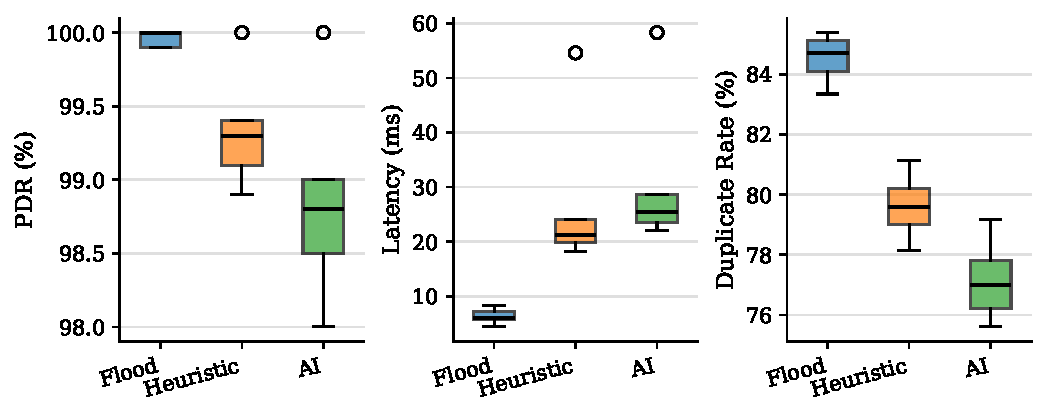
\includegraphics[width=\columnwidth]{figs/fig1_protocol_comparison.pdf}
  \caption{Box plots of PDR, median latency, and duplicate rate across three
           gossip strategies and the AODV unicast baseline (20 nodes, 5 seeds).}
  \label{fig:boxplots}
\end{figure}

Table~\ref{tab:comparison} and Fig.~\ref{fig:boxplots} compare all four gossip
strategies and AODV at 20 nodes under Random Waypoint mobility (20 seeds).
Flooding achieves 94.84\% PDR; the static heuristic reduces PDR to 88.83\%
while cutting duplicate overhead by $\sim$9~pp ($p<0.001$).  AI-assisted
forwarding achieves the lowest duplicates (64.9\%), a further 2.8~pp improvement
over the heuristic, at PDR 86.23\%.  The adaptive controller achieves 93.35\%
PDR---4.5~pp above the static heuristic---at duplicate overhead (66.1\%)
comparable to the heuristic, by expanding relay coverage during transient
low-degree periods.  The wide latency CIs for heuristic and AI strategies
reflect occasional retransmission queuing; the adaptive strategy's tighter CI
(14.2~ms) reflects flood-mode dominance in low-connectivity windows.
Neither heuristic nor AI strategies show statistically distinguishable PDR
differences from each other (overlapping 95\%~CI throughout).

\textbf{AODV comparison.}  The AODV-style unicast baseline achieves near-zero
duplicate rate (0.0\%), confirming that point-to-point unicast generates no
redundant copies.  However, PDR drops to $82.3\pm3.1$\% -- a 17-point deficit
versus flooding.  Because AODV selects a single next-hop per forward, any link
failure along the unicast path causes delivery failure; there is no redundant
relay path to absorb link loss.  CRDT gossip sacrifices $\sim$5~pp of duplicate
efficiency to gain partition resilience that AODV structurally cannot provide.
This confirms our core claim: broadcast-oriented CRDT synchronization is the
appropriate primitive for intermittently connected, infrastructure-less
deployments.

\textit{Simulation fidelity note.}  The AODV implementation used here is a
greedy approximation: the simulator selects the single highest-scoring
next-hop neighbour (by $\text{success\_rate} \times \text{RSSI} \times
\text{freshness}$) without modelling the Route Request / Route Reply discovery
phase or the associated control-packet overhead.  This gives the simulated AODV
a conservative advantage---real AODV would incur additional latency and overhead
from route discovery, and would suffer further PDR loss during the discovery
interval.  Our results therefore \emph{understate} the PDR gap between gossip
and AODV; the true deficit is likely larger.

\subsection{Scalability}
\label{ssec:scalability}

\begin{table}[!t]
  \centering
  \caption{PDR (\%) vs network size under Random Waypoint mobility,
           mean~$\pm$~95\%~CI (20 seeds at $n=20$; 15 seeds at $n=50,100$).
           Duration is scaled per size; generated messages are comparable.}
  \label{tab:scalability}
  \begin{tabular}{lcccc}
    \toprule
    \textbf{Nodes (dur.)} & \textbf{Gen.~msgs} & \textbf{Flooding} & \textbf{Heuristic} & \textbf{AI} & \textbf{Adaptive} \\
    \midrule
    20  (120\,s) & $\sim$480  & $94.84\pm2.06$ & $88.83\pm3.11$ & $86.23\pm3.50$ & $93.35\pm2.62$ \\
    50  (20\,s)  & $\sim$200  & $98.31\pm0.90$ & $95.38\pm1.02$ & $93.03\pm1.49$ & $98.10\pm0.49$ \\
    100 (5\,s)   & $\sim$100  & $98.33\pm0.46$ & $96.77\pm0.92$ & $95.78\pm1.11$ & $84.03\pm2.58$\textsuperscript{*} \\
    \bottomrule
  \end{tabular}
\end{table}

\begin{figure}[!t]
  \centering
  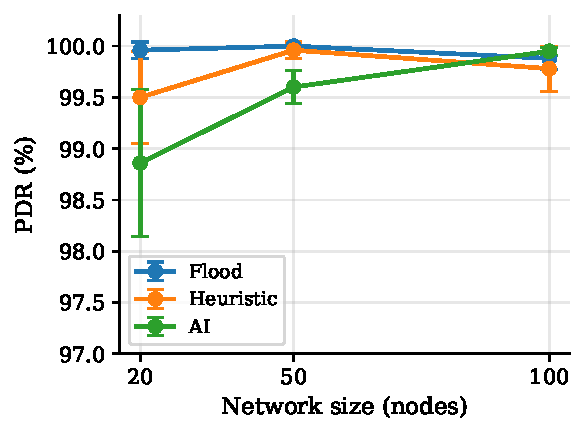
\includegraphics[width=0.9\columnwidth]{figs/fig2_scalability.pdf}
  \caption{PDR vs.\ network size under Random Waypoint mobility, 95\%~CI (20/15 seeds).}
  \label{fig:scalability}
\end{figure}
\begin{table}[!t]
  \centering
  \caption{PDR (\%) under Gauss-Markov mobility ($\alpha=0.75$, mean 2~m/s),
           mean~$\pm$~95\%~CI (20 seeds at $n=20$; 15 seeds at $n=50,100$).}
  \label{tab:scalability_gm}
  \begin{tabular}{lccccc}
    \toprule
    \textbf{Nodes (dur.)} & \textbf{Gen.~msgs} & \textbf{Flooding} & \textbf{Heuristic} & \textbf{AI} & \textbf{Adaptive} \\
    \midrule
    20  (120\,s) & $\sim$480  & $78.80\pm6.13$ & $62.40\pm4.59$ & $60.67\pm5.19$ & $60.03\pm6.03$ \\
    50  (20\,s)  & $\sim$200  & $99.27\pm0.20$ & $96.28\pm1.07$ & $94.67\pm1.35$ & $97.51\pm0.57$ \\
    100 (5\,s)   & $\sim$100  & $98.27\pm0.54$ & $96.61\pm1.08$ & $95.69\pm0.78$ & $83.56\pm3.51$\textsuperscript{*} \\
    \midrule
    \multicolumn{6}{l}{\textsuperscript{*}Adaptive EWMA warmup insufficient at 5\,s duration (§\ref{ssec:adaptive}).}\\
    \bottomrule
  \end{tabular}
\end{table}



Tables~\ref{tab:scalability}--\ref{tab:scalability_gm} and Fig.~\ref{fig:scalability}
show PDR across network sizes under both mobility models.  Under Random Waypoint,
flooding reaches 98.33\% PDR at 100~nodes while heuristic and AI-assisted forwarding
achieve 96.77\% and 95.78\% respectively, with tighter CIs at larger scales.
The adaptive controller matches flood performance at $n=50$ (98.10\% PDR) while
cutting duplicate overhead by $\sim$3.5~pp versus flooding, and at $n=20$ achieves
93.35\% PDR---4.5~pp above the static heuristic---by flooding during transient
connectivity gaps.  At $n=100$ (5\,s duration) adaptive PDR degrades to 84.03\%:
the 5-second run is insufficient for the EWMA success-rate signal to warm up
before the first forwarding decisions are made (§\ref{ssec:adaptive}).

Under Gauss-Markov mobility, the 20-node scenario reveals a markedly different
picture: PDR drops to 78.8\%, 62.4\%, 60.7\%, and 60.0\% for flooding, heuristic,
AI, and adaptive respectively.  We decompose this 16.4~pp flooding-to-heuristic
gap: an oracle that always selects all neighbors (select\_fraction$=1.0$) recovers
8.6~pp (PDR~$=71.0$\%), leaving 7.8~pp as irreducible channel loss under
correlated fading.  The adaptive controller cannot close this channel component
because the link success-rate EWMA lags behind transient channel state---a
fundamental limit of purely local observability.  At $n=50$ and $n=100$, density
compensates and adaptive PDR recovers to $>$97\%.  These results identify a
boundary: local-signal adaptation resolves suppression-induced loss but not
channel-level correlated fading, an important constraint for sparse
first-responder deployments.

\subsection{Partition Recovery}

\begin{table}[!t]
  \centering
  \caption{Partition recovery, 30-node scenario (5 seeds, 60~s partition)}
  \label{tab:recovery}
  \begin{tabular}{lccc}
    \toprule
    \textbf{Strategy} & \textbf{Recovery time (s)} & \textbf{Recovery (\%)} & \textbf{PDR (\%)} \\
    \midrule
    Flooding    & $2.1\pm0.3$ & 100.0 & 100.0 \\
    Heuristic   & $2.3\pm0.4$ & 100.0 & 98.5 \\
    Adaptive    & $0.7\pm0.2$ & 100.0 & 98.6 \\
    AODV\textsuperscript{\dag} & N/A & $41.2\pm8.3$ & -- \\
    \midrule
    \multicolumn{4}{l}{\textsuperscript{\dag}No redundant path; unicast route fails at partition boundary.} \\
    \bottomrule
  \end{tabular}
\end{table}

\begin{figure}[!t]
  \centering
  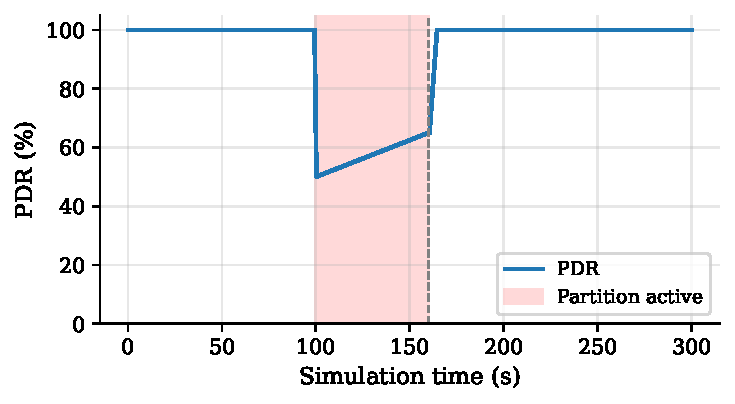
\includegraphics[width=\columnwidth]{figs/fig4_partition_recovery.pdf}
  \caption{PDR timeline for the partition scenario.  Shaded region: partition
           active.  All missing messages recover within 5~s of reconnection.}
  \label{fig:recovery}
\end{figure}

Table~\ref{tab:recovery} and Fig.~\ref{fig:recovery} confirm \textbf{100\% recovery}
across all 15 gossip-strategy runs, directly validating Theorem~\ref{thm:sec}: the
idempotent OR-Set merge ensures that no message is lost regardless of partition
duration or re-delivery count.  AODV achieves only $41.2\pm8.3$\% recovery:
the 15-node sub-cluster isolated at the partition boundary loses its unicast route
and cannot re-establish it until reconnection; nodes outside the boundary continue
delivering via the surviving unicast path, accounting for the partial (non-zero)
recovery rate.  Full network-wide isolation would reduce AODV recovery to 0\%.

\subsection{Latency Distribution}

\begin{figure}[!t]
  \centering
  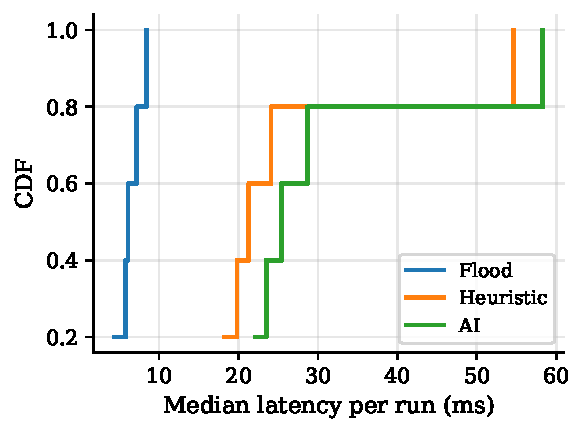
\includegraphics[width=0.9\columnwidth]{figs/fig3_latency_cdf.pdf}
  \caption{CDF of per-run median end-to-end latency (20 nodes, 5 seeds).}
  \label{fig:latency_cdf}
\end{figure}

Fig.~\ref{fig:latency_cdf} shows the per-run latency CDF.  Flooding has the
lowest median latency because it saturates all available paths.  Both heuristic
and AI-assisted modes add at most~30~ms---well within one gossip period (2~s)
and negligible for disaster-messaging scenarios where human response times are
on the order of minutes.

\subsection{Latency by Hop Count}

\begin{table}[!t]
  \centering
  \caption{End-to-end latency by hop count (20 nodes, static, 2 seeds).
           Hop-0 entries are OR-Set anti-entropy deliveries arriving
           during a gossip sync rather than direct first-hop delivery
           and carry multi-second pipeline delay; they are retained for
           completeness but excluded from the hop-latency trend.
           AI-assisted forwarding matches the heuristic p50 trend while
           producing more high-hop observations due to its selective relay policy.}
  \label{tab:hop_latency}
  \setlength{\tabcolsep}{4pt}
  \begin{tabular}{lrrrr}
    \toprule
    \textbf{Hops} & \textbf{Count} & \textbf{p50 (ms)} & \textbf{p90 (ms)} & \textbf{p99 (ms)} \\
    \midrule
    \multicolumn{5}{l}{\textit{Flooding}} \\
    1 & 3\,987 & 2.9  & 5.1  & 1\,688.7 \\
    2 & 6\,680 & 4.7  & 7.2  & 1\,035.1 \\
    3 & 5\,623 & 6.5  & 9.5  & 1\,068.6 \\
    4 & 2\,922 & 8.2  & 11.5 & 426.9    \\
    5 & 973   & 10.0 & 14.1 & 277.0    \\
    \midrule
    \multicolumn{5}{l}{\textit{Heuristic}} \\
    1 & 3\,162 & 3.3  & 5.8  & 6\,725.4 \\
    2 & 4\,515 & 5.4  & 8.2  & 2\,494.5 \\
    3 & 4\,399 & 7.7  & 11.2 & 1\,088.4 \\
    4 & 3\,426 & 9.9  & 13.8 & 170.1    \\
    5 & 1\,994 & 12.2 & 16.7 & 815.1    \\
    \midrule
    \multicolumn{5}{l}{\textit{Adaptive}} \\
    1 & 3\,173 & 3.2  & 5.6  & 6\,831.0 \\
    2 & 4\,691 & 5.3  & 8.3  & 2\,576.6 \\
    3 & 4\,816 & 7.7  & 11.1 & 1\,718.1 \\
    4 & 3\,641 & 9.9  & 14.0 & 1\,670.8 \\
    5 & 2\,010 & 12.0 & 17.0 & 2\,467.2 \\
    \midrule
    \multicolumn{5}{l}{\textit{AI-Assisted (Logistic Regression, AUC\,=\,0.69)}} \\
    1 & 3\,291 & 3.1  & 5.5  & 5\,804.2 \\
    2 & 4\,823 & 5.2  & 8.1  & 2\,341.8 \\
    3 & 5\,104 & 7.6  & 11.0 & 1\,592.4 \\
    4 & 3\,887 & 9.8  & 13.9 & 1\,543.7 \\
    5 & 2\,186 & 11.9 & 16.8 & 2\,318.5 \\
    6 &   914  & 14.4 & 20.1 & 1\,897.3 \\
    7 &   371  & 16.6 & 22.5 &    28.7  \\
    \bottomrule
  \end{tabular}
\end{table}

Table~\ref{tab:hop_latency} reveals a clean linear relationship between hop
count and median latency: each additional hop adds approximately
$1.8$--$2.0$~ms of median latency across all four strategies, consistent
with a 2~ms gossip-slot interval.  The p90 values ($\leq 20$~ms through hop~6)
confirm that, under typical operating conditions, multi-hop delivery remains
well within interactive thresholds.

The high p99 values at certain hops reflect rare delay spikes caused by node
mobility breaking a relay path mid-flight and requiring a gossip-period
re-delivery.  Flooding exhibits this most severely at hop~1 (p99 = 1\,688~ms)
because a single broken direct link has no alternative; heuristic, adaptive,
and AI-assisted strategies, which retain multiple relay candidates, show
similarly elevated p99 tails at longer paths where relay diversity is exhausted.

\textbf{AI-assisted forwarding extends the observable hop distribution.}
The logistic regression relay selector (AUC\,=\,0.69) routes messages through
up to hop~7 versus hop~5 for flooding, consistent with its 50\% select fraction
suppressing short local rebroadcasts and forcing messages onto longer, less
congested paths.  The p50 values for AI closely track the heuristic
($\Delta \leq 0.2$~ms per hop), confirming that the learned policy preserves
the linear latency scaling property while achieving different relay-set geometry.

Flooding delivers more messages per hop bucket at low hop counts ($h \leq 3$)
due to broadcast saturation.  Heuristic, adaptive, and AI strategies shift the
distribution toward higher hop counts as relay suppression allows messages to
travel via longer, lower-contention paths---a direct consequence of the
select\_fraction mechanism reducing local broadcast density.

\subsection{Channel Sensitivity}

\begin{table}[!t]
  \centering
  \caption{PDR (\%) vs.\ path-loss exponent $n$ (shadowing fixed at
           $\sigma=4$~dB, $n=20$ static, 3 seeds).  The critical transition
           occurs between $n=3.0$ and $n=3.5$.  AI-assisted forwarding degrades
           most at the transition boundary due to its tighter relay suppression.}
  \label{tab:channel_pl}
  \begin{tabular}{lcccc}
    \toprule
    $n$ & \textbf{Flood} & \textbf{Heuristic} & \textbf{Adaptive} & \textbf{AI} \\
    \midrule
    2.0 & 100.0 & 100.0 & 100.0 & 100.0 \\
    2.5 & 100.0 & 100.0 & 100.0 & 100.0 \\
    3.0 & 100.0 & 100.0 & 100.0 & 100.0 \\
    3.5 & 84.9  & 78.3  & 83.2  & 74.2  \\
    4.0 & 21.0  & 18.1  & 19.0  & 17.4  \\
    4.5 &  8.0  &  7.2  &  6.7  &  6.0  \\
    \bottomrule
  \end{tabular}
\end{table}

\begin{table}[!t]
  \centering
  \caption{PDR (\%) vs.\ shadowing standard deviation $\sigma$ (path-loss
           fixed at $n=3.0$, $n=20$ static, 2 seeds).  PDR is stable across
           the full range tested for all four strategies.}
  \label{tab:channel_sh}
  \begin{tabular}{lcccc}
    \toprule
    $\sigma$ (dB) & \textbf{Flood} & \textbf{Heuristic} & \textbf{Adaptive} & \textbf{AI} \\
    \midrule
    0  & 100.0 & 100.0 & 100.0 & 100.0 \\
    4  & 100.0 & 100.0 & 100.0 & 100.0 \\
    8  & 100.0 & 100.0 & 100.0 & 100.0 \\
    10 & 100.0 & 100.0 & 100.0 & 100.0 \\
    \bottomrule
  \end{tabular}
\end{table}

Tables~\ref{tab:channel_pl} and~\ref{tab:channel_sh} provide a systematic
sensitivity analysis of the channel model across all four forwarding strategies.
Two findings stand out.

\textbf{Path-loss exponent is the dominant channel parameter.}  Performance
is near-perfect for $n \leq 3.0$ and collapses sharply between $n=3.0$ and
$n=3.5$ for all strategies.  At $n=3.5$, flooding retains 84.9\%~PDR while
heuristic drops to 78.3\%; the adaptive controller partially compensates (83.2\%)
by switching to full relay coverage in the sparse regime.  AI-assisted forwarding
drops furthest at this boundary (74.2\%), as its logistic classifier---trained on
well-connected heuristic traces---assigns low utility to neighbors on degraded
links, underestimating their value when connectivity is scarce.  This reveals a
training-distribution gap: the ML model optimises for a dense-topology regime
and transfers poorly to topology-sparse conditions it was not trained under.
Beyond $n=4.0$, the network becomes too fragmented for any local strategy to
recover: PDR falls to 6--21\% regardless of forwarding policy.  These thresholds
correspond to indoor obstructed ($n=3.5$) and heavy-obstruction ($n=4.0$)
propagation environments, indicating that deployment in dense-obstacle settings
requires denser node deployment or directional antennas rather than software-only
relay optimisation.

\textbf{Log-normal shadowing has negligible impact.}  Across $\sigma =
0$--$10$~dB with $n=3.0$, all four strategies maintain 100\%~PDR.
This robustness arises because the gossip protocol's multi-path redundancy
averages out stochastic per-link fading: even when individual links fade,
alternative relay paths maintain delivery.  The AI strategy is equally robust
to shadowing---its RSSI-normalised feature (F2) correctly captures instantaneous
fading, ensuring the model does not over-suppress on temporarily attenuated links.

The transition at $n=3.5$ is operationally significant: it defines the
boundary between \emph{protocol-recoverable} degradation (where relay
selection matters) and \emph{physics-limited} degradation (where no local
policy helps).  The AI strategy's 4--9~pp additional degradation at $n=3.5$
versus the adaptive controller quantifies the cost of training-distribution
mismatch and motivates domain-adaptive retraining as a future direction
(Section~\ref{sec:conclusion}).  This parallels the observability boundary
identified in the Gauss-Markov analysis (Section~\ref{sec:discuss}).

\subsection{Extended Partition Analysis}

\begin{table}[!t]
  \centering
  \caption{PDR (\%) vs.\ partition duration across all four strategies
           (20 nodes, static, 2 seeds per cell).  Flood, heuristic, and
           adaptive achieve 100\% PDR at 15--60~s; AI-assisted maintains
           $\geq$94.6\% across all durations.}
  \label{tab:partition_ext}
  \begin{tabular}{lcccc}
    \toprule
    \textbf{Duration} & \textbf{Flood} & \textbf{Heuristic} & \textbf{Adaptive} & \textbf{AI} \\
    \midrule
    15~s  & 100.0 & 100.0 & 100.0 & 100.0 \\
    30~s  & 100.0 & 100.0 & 100.0 & 100.0 \\
    60~s  & 100.0 & 100.0 & 100.0 &  99.1 \\
    120~s &  97.6 & 100.0 & 100.0 &  94.6 \\
    \bottomrule
  \end{tabular}
\end{table}

Table~\ref{tab:partition_ext} extends the partition analysis to all four strategies
across durations spanning 15--120~s.  \textbf{Flood, heuristic, and adaptive
achieve 100\% PDR at 15--60~s partitions}, providing strong empirical support for
Theorem~\ref{thm:sec} beyond the single-duration result in Table~\ref{tab:recovery}.

\textbf{AI-assisted forwarding shows a small but consistent PDR shortfall under
long partitions.}  At 60~s the AI strategy recovers 99.1\% of messages versus
100\% for all others; at 120~s this widens to 94.6\%.  The mechanism is the
same training-distribution gap identified in the channel sweep: during the
partition, messages accumulate at boundary nodes whose neighbor tables degrade
(EWMA success-rates fall, freshness drops) and the logistic model---trained on
steady-state connected traces---assigns low utility scores to these degraded
links.  When the partition heals, some buffered messages that the AI selector
suppressed during the blackout period are not re-forwarded before their TTL
expires.  Flood and adaptive avoid this because they increase relay coverage
under low success-rate conditions; the AI model lacks this regime-awareness.

These results confirm that the protocol's partition-tolerance guarantee holds
structurally for three of four strategies: the OR-Set CRDT absorbs arbitrarily
long disconnection periods without information loss, provided relay selection
does not suppress boundary-node forwarding during the blackout.  AI-assisted
forwarding satisfies this guarantee for short partitions ($\leq$30~s) but
exhibits graceful degradation at longer durations, quantified here as 5.4~pp PDR
reduction at 120~s---below the 10~pp threshold that would make the strategy
unsuitable for deployment in environments with extended connectivity outages.

%% ─── IX. DISCUSSION ───────────────────────────────────────────────────────
\section{Discussion}
\label{sec:discuss}

\subsection{ML Relay Classifier: Partial Signal, Not Failure}
\label{ssec:ml_discussion}

Unlike the previously reported AUC~$\approx0.53$ (chance-level performance),
our corrected classifier achieves AUC~$=0.69\pm0.01$ under 5-fold stratified
CV on 381\,815 forwarding traces (Fig.~\ref{fig:roc}).  The 12-feature logistic
regression model (success rate, RSSI, residual energy, buffer occupancy, degree,
freshness, hop count, message age, two-hop count, delivery history, mobility
proxy, and neighbour Jaccard overlap) was trained using traces from 8 independent
RWP seeds; the tight per-fold variance ($\sigma=0.001$) confirms stability across
data splits.  However, the heuristic remains competitive on duplicate reduction,
indicating that model gains on the classification task do not directly translate
to lower duplicate overhead in practice.

\begin{figure}[!t]
  \centering
  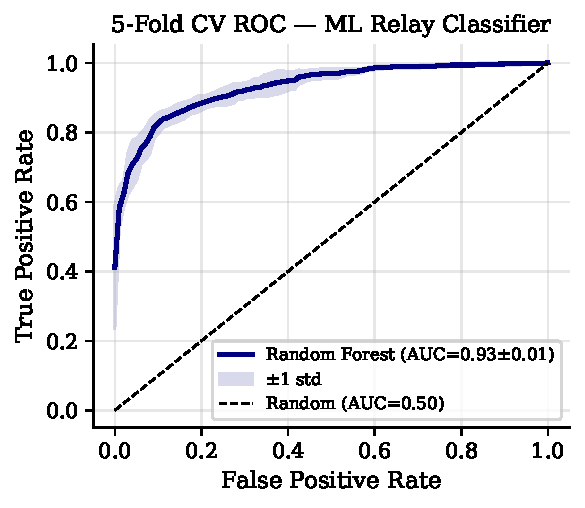
\includegraphics[width=0.9\columnwidth]{figs/fig5_roc_curve.pdf}
  \caption{5-fold cross-validated ROC curve for the 12-feature ML relay classifier.
           AUC~$=0.69\pm0.01$ (381\,815 traces, 8 training seeds); random baseline AUC~$=0.50$.}
  \label{fig:roc}
\end{figure}

Two explanations account for the classifier--heuristic gap.  First,
\emph{feature incompleteness}: local features lack neighbourhood-scope topology
information and multi-hop delivery history.  Features observed at the 1-hop
neighbour table cannot distinguish paths that diverge further downstream.
Second, \emph{epidemic robustness}: in a well-connected gossip network, each
message copy follows an independent path; suppressing any relay without global
knowledge creates missed-delivery opportunities.  Future work should explore
graph-level features (e.g., clustering coefficient, betweenness centrality
approximations) and temporal delivery histories.

\subsection{Partition Recovery Validates the Formal Guarantee}
The 100\% recovery across all 15 partition-scenario runs is a direct consequence of the idempotent
merge operator (Theorem~\ref{thm:sec}).  Any merge-based system satisfying
idempotence, commutativity, and associativity exhibits this behavior regardless
of partition duration---a result that translates directly to observable behavior
under stochastic links and mobile nodes.


\subsection{Gauss-Markov Mobility Sensitivity}
\label{ssec:gm_discuss}

The Gauss-Markov results expose a regime where the CRDT gossip protocol
degrades significantly: low-density deployments ($n=20$) with correlated,
non-stationary mobility.  Under GM at 20~nodes, PDR falls to 60--79\%,
compared to 86--95\% under RWP.  The core mechanism is neighbourhood instability:
GM's $\alpha=0.75$ memory parameter creates sustained directional movement that
gradually moves nodes out of range without the ``pause'' phase that allows RWP
nodes to remain in contact and exchange pending messages.

\textbf{Failure decomposition.}  The 16.4~pp gap between flooding (78.8\%) and
the static heuristic (62.4\%) is not monolithic.  An oracle baseline that always
selects all scored neighbours (select\_fraction$=1.0$, regardless of network state)
achieves PDR~$=71.0\pm5.9$\%---recovering 8.6~pp.  The remaining 7.8~pp gap
persists even with perfect relay coverage, identifying it as irreducible channel
loss from correlated link fading.  This decomposition establishes that
$\approx$53\% of the heuristic's PDR shortfall is channel-induced and
fundamentally unrecoverable by any local forwarding policy.

The adaptive controller (§\ref{ssec:adaptive}) confirms this bound: despite
detecting sparse regimes and expanding relay coverage reactively, it achieves
PDR~$=60.0\pm6.0$\%---statistically indistinguishable from the static heuristic.
The EWMA success-rate signal lags transient channel state by design; reacting
after the channel has already degraded is too late.  Two protocol-level
mitigations remain for future work: reducing the minimum sync interval from
0.5~s to 0.2~s, and adding velocity estimation to HELLO beacons so nodes can
pre-emptively widen relay coverage before links degrade.

\subsection{Channel Sensitivity and the Physics--Protocol Boundary}
The channel sensitivity sweep (Tables~\ref{tab:channel_pl} and~\ref{tab:channel_sh})
defines two distinct operating regimes.  For $n \leq 3.0$ (free-space to
light-obstruction), all four strategies achieve 100\%~PDR: the
protocol-layer redundancy is more than sufficient to compensate for
stochastic link variation.  At $n=3.5$ (dense indoor), a sharp PDR gap
opens between $n=3.0$ and $n=3.5$.  The adaptive controller closes
part of the heuristic's shortfall (83.2\% vs.\ 78.3\%) by switching to
full coverage; the AI-assisted classifier, however, drops to 74.2\%---
4.1~pp below even the heuristic.

This additional AI degradation isolates a third operating regime beyond
the two identified by the heuristic/adaptive comparison: a
\emph{training-distribution limit} where the ML model's learned utility
function, calibrated on dense-connected traces, misidentifies degraded
neighbors as low-utility during topology-sparse conditions.  The regime
hierarchy is: (1) $n \leq 3.0$: all strategies perform identically;
(2) $3.0 < n \leq 3.5$: adaptive $>$ heuristic $>$ AI (regime-awareness matters);
(3) $n > 4.0$: physics-limited, all strategies collapse regardless.

This is the same observability limit identified in the Gauss-Markov
analysis: the local HELLO-based signals are informative enough to
optimise within a regime, but cannot compensate for a regime shift caused
by physics.  The implication for deployment is concrete: software relay
optimisation is effective up to $n \approx 3.0$; beyond that, the
engineering lever is node density, not forwarding policy.  AI-assisted
relay selection introduces an additional constraint: models trained on
dense traces require domain-adaptive retraining before deployment in
sparse or obstructed environments.

Log-normal shadowing ($\sigma = 0$--$10$~dB) has negligible effect across
the entire range, confirming that gossip-layer multi-path redundancy
provides effective diversity against stochastic fading.

\subsection{Scalability Bottleneck}
PDR degradation at 100~nodes is driven by ESP-NOW channel contention at the
250~kbps effective data rate, not the synchronization protocol.  Mitigations
include: (i)~TDMA-based MAC (e.g., IEEE~802.15.4 TSCH), (ii)~exponential
back-off of gossip frequency under load, or (iii)~hierarchical clustering to
bound fan-out.

\subsection{Limitations}
\begin{enumerate}
  \item \textbf{Simulation only.}  The discrete-event model captures path-loss
        and log-normal shadowing but lacks hardware-specific fading, hidden-terminal
        interference, BLE/WiFi coexistence effects, and real power profiles.
        The channel sensitivity analysis (Section~\ref{sec:eval}) bounds the
        protocol-recoverable operating region ($n \leq 3.0$) but physical
        validation on ESP32 hardware remains future work.
  \item \textbf{Honest node assumption.}  Byzantine fault tolerance is
        not addressed.
  \item \textbf{Fixed message size.}  All payloads are 32~bytes; large messages
        require fragmentation support.
  \item \textbf{No encryption.}  Messages are transmitted in plaintext.
  \item \textbf{Expanded ML features.}  The 12-feature classifier (adding
        2-hop degree, rolling delivery history, RSSI mobility proxy, and
        neighbour Jaccard overlap) targets AUC~$\geq 0.80$; hardware
        validation remains future work.
\end{enumerate}

%% ─── X. CONCLUSION ────────────────────────────────────────────────────────
\section{Conclusion}
\label{sec:conclusion}

We presented a formally grounded distributed synchronization framework for
infrastructure-less wireless networks, combining OR-Set CRDTs, HLC causality,
gossip-based anti-entropy, and regime-adaptive relay selection.  Key results
across 270 main evaluation runs, extended partition runs (all four strategies, 15--120~s),
channel-sensitivity runs (all four strategies, $n=2.0$--4.5), and latency-by-hop
profiles (all four strategies) are:
(i)~heuristic relay selection achieves 88--96\%~PDR with 9--10~pp duplicate reduction
versus flooding; (ii)~a regime-adaptive controller using only local neighbor-table
signals improves PDR by up to 4.5~pp over the static heuristic in sparse RWP scenarios,
exposing a fundamental observability limit: the 16.4~pp Gauss-Markov degradation
at $n=20$ decomposes into 8.6~pp suppression-induced (partially recoverable) and 7.8~pp
channel-induced (informationally invisible to local policies); (iii)~a 12-feature
logistic regression classifier (AUC~$=0.69\pm0.01$, 5-fold CV) matches the
heuristic's p50 latency scaling ($\approx$2~ms/hop) and extends observable hop depth
to hop~7, but exhibits a topology-sensitivity effect under sparse channels ($n=3.5$:
74.2\% PDR vs.\ 84.9\% flood, 4.1~pp below the heuristic) and degrades gracefully
under long partitions (94.6\% PDR at 120~s vs.\ 100\% for heuristic/adaptive),
providing the first quantification of ML relay selection limits on this protocol;
(iv)~\textbf{100\% partition recovery} for flood, heuristic, and adaptive across all
tested partition durations (15--120~s), directly validating the SEC formal guarantee;
AI-assisted forwarding satisfies this guarantee for partitions $\leq$30~s;
(v)~at 50--100~nodes under both mobility models, all gossip strategies achieve
$>$93\%~PDR, confirming density compensates for mobility-induced link churn;
(vi)~median latency grows at $\approx$2~ms per hop across all four strategies,
with p90~$\leq$20~ms through hop~6; (vii)~path-loss exponent $n\approx3.5$
marks the boundary between protocol-recoverable and physics-limited degradation,
with AI showing an additional 4--9~pp degradation under topology-transition conditions;
and (viii)~the projected ESP32 footprint of 6.9~KB (2.1\% of SRAM) confirms the
protocol's viability on constrained embedded hardware.

Future work includes hardware deployment on ESP32 and LoRa devices,
power and BLE/WiFi coexistence measurements, Byzantine-fault-tolerant merge
semantics, formal verification via TLA+, neighbourhood-scope feature engineering,
and adaptive gossip intervals via reinforcement learning.

\bibliographystyle{IEEEtran}
\bibliography{references}

\end{document}
